\chapter{\LTLfToDFA}\label{ch:ltlf2dfa}
In this chapter we will present \href{https://github.com/Francesco17/LTLf2DFA}{\LTLfToDFA}, a software package  written in Python. 

\section{Introduction}\label{sec:intro}
\LTLfToDFA is a Python tool that processes a given \LTLf formula (with past and future operators) and generates the corresponding minimized \DFA using \MONA\citep{mona1998}. In addition, it offers the possibility to compute the \DFA with or without the \declare assumption \citep{DeGiacomo:2014:RLF:2893873.2894033}.
The main features provided by the library are:
\begin{itemize}
\item parsing an \LTLf formula with past or future operators;
\item translation of an \LTLf formula to \MONA program;
\item conversion of an \LTLf formula to \DFA automaton.
\end{itemize}
\LTLfToDFA can be used with Python>=3.6 and has the following dependencies:
\begin{itemize}
\item \href{http://www.dabeaz.com/ply/ply.html}{PLY}, a pure-Python implementation of the popular compiler construction tools \href{http://dinosaur.compilertools.net/}{Lex and Yacc}. It has been employed for parsing the input \LTLf formula;
\item \href{http://www.brics.dk/mona/}{\MONA}, a C++ tool that translates formulas to \DFA. It has been used for the generation of the \DFA;
\item \href{https://pypi.org/project/dotpy/}{Dotpy}, a Python library able to parse and modify \texttt{.dot} files. It has been utilized for post-processing the \MONA output.
\end{itemize}
The package is available to download on \href{https://pypi.org/project/ltlf2dfa/}{PyPI} and you can install it by typing in the terminal:
\begin{lstlisting}[language=bash]
pip install ltlf2dfa
\end{lstlisting}
All the code is available online on GitHub\footnote{https://github.com/Francesco17/LTLf2DFA}, it is open source and it is released under the \href{https://github.com/Francesco17/LTLf2DFA/blob/master/LICENSE}{MIT License}.
Moreover, \LTLfToDFA can also be tried online at \href{ltlf2dfa.diag.uniroma1.it}{ltlf2dfa.diag.uniroma1.it}.
\section{Package Structure}
The structure of the \LTLfToDFA package is quite simple. It consists of a main folder called \texttt{ltlf2dfa/} which hosts the most important library's modules:
\begin{itemize}
\item \texttt{Lexer.py}, where the Lexer class is defined;
\item \texttt{Parser.py}, where the Parser class is defined;
\item \texttt{Translator.py}, where the main APIs for the translation are defined;
\item \texttt{DotHandler.py}, where we the \MONA output is post-processed.
\end{itemize}
In the following paragraphs we will explore each module in detail.
\subsection{Lexer.py}
In the \texttt{Lexer.py} module we can find the declaration of the \texttt{MyLexer} class which is in charge of handling the input string and tokenizing it. Indeed, it implements a tokenizer that splits the input string into declared individual tokens.
To our extent, we have defined the class as in Listing \ref{code:ltlf2dfa-lexer}
\begin{lstlisting}[language=Python, style=Python, escapechar = £, label={code:ltlf2dfa-lexer}, caption={\texttt{Lexer.py} module}]
import ply.lex as lex

class MyLexer(object):

    reserved = {
        'true':     'TRUE',
        'false':    'FALSE',
        'X':        'NEXT',
        'U':        'UNTIL',
        'E':        'EVENTUALLY',
        'G':        'GLOBALLY',
        'Y':        'PASTNEXT', #PREVIOUS
        'S':        'PASTUNTIL', #SINCE
        'O':        'PASTEVENTUALLY', #ONCE
        'H':        'PASTGLOBALLY'
    }
    # List of token names.   This is always required
    tokens = (
        'TERM',
        'NOT',
        'AND',
        'OR',
        'IMPLIES',
        'DIMPLIES',
        'LPAR',
        'RPAR'
    ) + tuple(reserved.values())

    # Regular expression rules for simple tokens
    t_TRUE = r'T'
    t_FALSE = r'F'
    t_AND = r'\&'
    t_OR = r'\|'
    t_IMPLIES = r'\->'
    t_DIMPLIES = r'\<->'
    t_NOT = r'\~'
    t_LPAR = r'\('
    t_RPAR = r'\)'
    # FUTURE OPERATORS
    t_NEXT = r'X'
    t_UNTIL = r'U'
    t_EVENTUALLY = r'E'
    t_GLOBALLY = r'G'
    # PAST OPERATOR
    t_PASTNEXT = r'Y'
    t_PASTUNTIL = r'S'
    t_PASTEVENTUALLY = r'O'
    t_PASTGLOBALLY = r'H'

    t_ignore = r' '+'\n'

    def t_TERM(self, t):£\label{line:lexer-term}£
        r'[a-z]+'
        t.type = MyLexer.reserved.get(t.value, 'TERM')
        return t  # Check for reserved words

    def t_error(self, t):
        print("Illegal character '%s' in the input formula" % t.value[0])
        t.lexer.skip(1)

    # Build the lexer
    def build(self,**kwargs):
        self.lexer = lex.lex(module=self, **kwargs)
\end{lstlisting}
Firstly, we have defined the reserved words within a dictionary so to match each reserved word with its identifier.
Secondly, we have defined the tokens list with all possible tokens that can be produced by the lexer. This tokens list is always required for the implementation of a lexer.
Then, each token has to be specified by writing a regular expression rule. If the token is simple it can be specified using only a string. Otherwise, for non trivial tokens we have to write the regular expression in a class method as for our token \texttt{TERM} in line \ref{line:lexer-term}. In that case, defining the token rule as a method is also useful when we would like to perform other actions. After that, we have a method to handle unrecognized tokens and, finally, we have written the function that builds the lexer.
\subsection{Parser.py}
In the \texttt{Parser.py} module we can find the declaration of \texttt{MyParser} class which implements the parsing component of \texttt{PLY}. The \texttt{MyParser} class operates after the Lexer has split the input string into known tokens. The main feature of the parser is to interpret and build the appropriate data structure for the given input. To this extent, the most important aspect of a parser is the definition of the \textit{syntax}, usually specified in terms of a BNF\footnote{The Backus–Naur form is a notation technique for context-free grammars.} grammar, that should be unambiguous. Furthermore, \texttt{Yacc}, the parsing component of \texttt{PLY}, implements a parsing technique known as LR-parsing or shift-reduce parsing. In particular, this parsing technique works on a bottom up fashion that tries to recognize the right-hand-side of various grammar rules. Whenever a valid right-hand-side is found in the input, the appropriate action code is triggered and the grammar symbols are replaced by the grammar symbol on the left-hand-side and so on until there is no more rule to apply. The parser implementation is shown in Listing \ref{code:ltlf2dfa-parser}
\begin{lstlisting}[language=Python, style=Python, label={code:ltlf2dfa-parser}, caption={\texttt{Parser.py} module}]
import ply.yacc as yacc
from ltlf2dfa.Lexer import MyLexer

class MyParser(object):

    def __init__(self):
        self.lexer = MyLexer()
        self.lexer.build()
        self.tokens = self.lexer.tokens
        self.parser = yacc.yacc(module=self)
        self.precedence = (

            ('nonassoc', 'LPAR', 'RPAR'),
            ('left', 'AND', 'OR', 'IMPLIES', 'DIMPLIES', 'UNTIL', \
             'PASTUNTIL'),
            ('right', 'NEXT', 'EVENTUALLY', 'GLOBALLY', \
            'PASTNEXT', 'PASTEVENTUALLY', 'PASTGLOBALLY'),
            ('right', 'NOT')
        )

    def __call__(self, s, **kwargs):
        return self.parser.parse(s, lexer=self.lexer.lexer)

    def p_formula(self, p):
        '''
        formula : formula AND formula
                 | formula OR formula
                 | formula IMPLIES formula
                 | formula DIMPLIES formula
                 | formula UNTIL formula
                 | formula PASTUNTIL formula
                 | NEXT formula
                 | EVENTUALLY formula
                 | GLOBALLY formula
                 | PASTNEXT formula
                 | PASTEVENTUALLY formula
                 | PASTGLOBALLY formula
                 | NOT formula
                 | TRUE
                 | FALSE
                 | TERM
        '''

        if len(p) == 2: p[0] = p[1]
        elif len(p) == 3:
            if p[1] == 'E': # E(a) == true UNITL A
                p[0] = ('U','T', p[2])
            elif p[1] == 'G': # G(a) == not(eventually (not A))
                p[0] = ('~',('U', 'T', ('~',p[2])))
            elif p[1] == 'O': # O(a) = true SINCE A
                p[0] = ('S','T', p[2])
            elif p[1] == 'H': # H(a) == not(pasteventually(not A))
                p[0] = ('~',('S', 'T', ('~',p[2])))
            else:
                p[0] = (p[1], p[2])
        elif len(p) == 4:
            if p[2] == '->':
                p[0] = ('|', ('~', p[1]), p[3])
            elif p[2] == '<->':
                p[0] = ('&', ('|', ('~', p[1]), p[3]), ('|', ('~', p[3]),\
                p[1]))
            else:
                p[0] = (p[2],p[1],p[3])
        else: raise ValueError


    def p_expr_group(self, p):
        '''
        formula : LPAR formula RPAR
        '''
        p[0] = p[2]

    def p_error(self, p):
        raise ValueError("Syntax error in input! %s" %str(p))
\end{lstlisting}
As we can see, as soon as the parser is instantiated it builds the lexer, gets the tokens and defines their precedence if needed. Then, we have defined methods of the \texttt{MyParser} class that are in charge of constructing the syntax tree structure from tokens found by the lexer in the input string. In our case, we have chosen to use as data structure a tuple of tuples as it is the one of the simplest data structure in Python. In general, a tuple of tuples represents a tree where each node represents an item present in the formula.

For instance, the \LTLf formula $\varphi= G(a \rightarrow X b)$ is represented as $('\thicksim', ('U', 'T', ('\thicksim',('|', ('\thicksim', 'a'), ('X', 'b')))))$ and it corresponds to a tree as the one depicted in Figure \ref{fig:formula-syntax-tree}.
\begin{figure}[h]
	\centering
	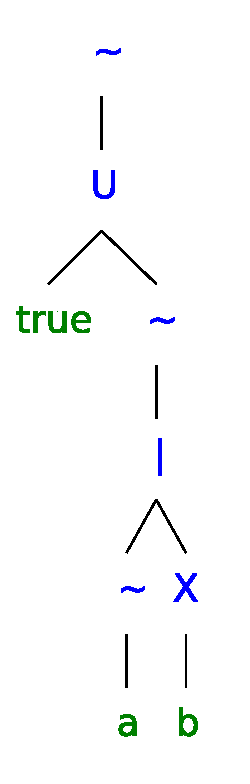
\includegraphics[height=15em, width=7.5em]{images/formula-syntax-tree}
	\caption{The syntax tree generated for the formula $"G(a \thicksim Xb)"$. Symbols are in green while operators are in blue.}
	\label{fig:formula-syntax-tree}
\end{figure}
Finally, as in the \texttt{MyLexer} class, we have to handle errors defining a specific method.

\LTLfToDFA can be used just for the parsing phase of an 	\LTLf formula as shown in Listing \ref{code:ltlf2dfa-only-parsing}.
\begin{lstlisting}[language=Python, style=Python, label={code:ltlf2dfa-only-parsing}, caption={How to use only the parsing phase of \LTLfToDFA.}]
from ltlf2dfa.Parser import MyParser

formula = "G(a->Xb)"
parser = MyParser()
parsed_formula = parser(formula)

print(parsed_formula) # syntax tree as tuple of tuples
\end{lstlisting}
\subsection{Translator.py}
The \texttt{Translator.py} module contains the majority of APIs that the \LTLfToDFA package exposes. Indeed, this module consists of a \texttt{Translator} class which concerns the core feature of the package: the translation of an \LTLf  formula into a \DFA. Since the package takes advantage of the \MONA tool for the formula conversion, the \texttt{Translator} class has to translate first the given formula into the syntax recognized by \MONA, then create the input program for \MONA and, finally, invoke \MONA to get back the resulting \DFA in the Graphviz\footnote{Graphviz is open source graph visualization software. For further details see \href{https://www.graphviz.org}{https://www.  .org}} format. 
The main methods of the \texttt{Translator} class are:
\begin{itemize}
\item \texttt{translate()}, which starting from the formula syntax tree generated (Figure \ref{fig:formula-syntax-tree}) in the parsing phase translates it into a string using the syntax of \MONA;
\item \texttt{createMonafile(flag)}, which, as the name suggests, creates the program \textit{.mona} that will be given as input to \MONA. The flag parameter is going to be \texttt{True} of \texttt{False} whether we need to compute also \declare  assumptions or not;
\item \texttt{invoke\_mona()}, which invokes \MONA in order to obtain the \DFA.
\end{itemize}
Now we will go into details of the methods stated above showing their implementation.
\subsubsection{The \texttt{translate} method}
The \texttt{translate} method is a crucial step towards reaching a good result and performance. Formally, the translation procedure from an \LTLf formula to the \MONA syntax is done passing through \FOL as shown in \ref{eq:translation-procedure}.
\begin{equation}\label{eq:translation-procedure}
\textsc{LTL}_f \rightarrow \textsc{FOL} \rightarrow \textsc{MONA}
\end{equation}
The former translation from \LTLf to \FOL is done accordingly to \citep{de2013linear}, while the latter follows from \citep{monamanual2001}.
In Listing \ref{code:ltlf2dfa-translate-method} we can see the translation's implementation. Three dots $\dots$ represent omitted code.
\begin{lstlisting}[language=Python, style=Python, escapechar = £,  label={code:ltlf2dfa-translate-method}, caption={The \texttt{translate} method.}]
import ...

class Translator:
    ...
    
    def translate(self):
        self.translated_formula = translate_bis(self.parsed_formula, \
        var='v_0')+";\n"

   ...

def translate_bis(formula_tree, var):£\label{line:translate_bis}£
    if type(formula_tree) == tuple:
        #enable this print to see the tree pruning
        # print(self.parsed_formula)
        # print(var)
        if formula_tree[0] == '&':
            # print('computed tree: '+ str(self.parsed_formula))
            if var == 'v_0':
                a = translate_bis(formula_tree[1], '0')
                # a = translate_bis(self.parsed_formula[1], '0')
                b = translate_bis(formula_tree[2], '0')
            else:
                a = translate_bis(formula_tree[1], var)
                b = translate_bis(formula_tree[2], var)
            if a == 'false' or b == 'false':
                return 'false'
            elif a == 'true':
                if b == 'true': return 'true'
            elif b == 'true': return a
            else: return '('+a+' & '+b+')'
        elif formula_tree[0] == '|':
            # print('computed tree: '+ str(self.parsed_formula))
            if var == 'v_0':
                a = translate_bis(formula_tree[1], '0')
                b = translate_bis(formula_tree[2], '0')
            else:
                a = translate_bis(formula_tree[1], var)
                b = translate_bis(formula_tree[2], var)
            if a == 'true' or b == 'true':
                return 'true'
            elif a == 'false':
                if b == 'true': return 'true'
                elif b == 'false': return 'false'
                else: return b
            elif b == 'false': return a
            else: return '('+a+' | '+b+')'
        elif formula_tree[0] == '~':
            # print('computed tree: '+ str(self.parsed_formula))
            if var == 'v_0': a = translate_bis(formula_tree[1], '0')
            else: a = translate_bis(formula_tree[1], var)
            if a == 'true': return 'false'
            elif a == 'false': return 'true'
            else: return '~('+ a +')'
        elif formula_tree[0] == 'X':
            # print('computed tree: '+ str(self.parsed_formula))
            new_var = _next(var)
            a = translate_bis(formula_tree[1],new_var)
            if var == 'v_0':
                return '('+ 'ex1 '+new_var+': '+ new_var +' = 1 '+ '& '+ \
                a +')'
            else:
                return '('+ 'ex1 '+new_var+': '+ new_var +' = '+ var + \
                ' + 1 '+ '& '+ a +')'
        elif formula_tree[0] == 'U':
            # print('computed tree: '+ str(self.parsed_formula))
            new_var = _next(var)
            new_new_var = _next(new_var)
            a = translate_bis(formula_tree[2],new_var)
            b = translate_bis(formula_tree[1],new_new_var)

            if var == 'v_0':
                if b == 'true': return '( '+ 'ex1 '+new_var+': 0 <= '+ \
                new_var+' & '+ new_var+' <= max($) & '+ a +' )'
                elif a ==  'true': return '( '+ 'ex1 '+new_var+': 0 <= '+ \
                new_var+' & '+new_var+' <= max($) & all1 '+ \
                new_new_var+': 0 <= '+new_new_var+' & '+ \
                new_new_var+' < '+new_var+' => '+b+' )'
                elif a == 'false': return 'false'
                else: return '( '+ 'ex1 '+new_var+': 0 <= '+new_var+ \
                ' & '+new_var+' <= max($) & '+ a +' & all1 '+ \
                new_new_var+': 0 <= '+new_new_var+' & '+ \
                new_new_var+' < '+new_var+' => '+b+' )'
            else:
                if b == 'true': return '( '+ 'ex1 '+new_var+': '+var+ \
                ' <= '+new_var+' & '+new_var+' <= max($) & '+ a +' )'
                elif a ==  'true': return '( '+ 'ex1 '+new_var+': '+var+ \
                ' <= '+new_var+' & '+new_var+' <= max($) & all1 '+ \ 
                new_new_var+': '+var+' <= '+new_new_var+' & '+ \ 
                new_new_var+' < '+new_var+' => '+b+' )'
                elif a == 'false': return 'false'
                else: return '( '+ 'ex1 '+new_var+': '+var+' <= '+ \ 
                new_var+' & '+new_var+' <= max($) & '+ a + \
                ' & all1 '+new_new_var+': '+var+' <= '+new_new_var+\
                ' & '+new_new_var+' < '+new_var+' => '+b+' )'
        elif formula_tree[0] == 'Y':
            # print('computed tree: '+ str(self.parsed_formula))
            new_var = _next(var)
            a = translate_bis(formula_tree[1],new_var)
            if var == 'v_0':
                return '('+ 'ex1 '+new_var+': '+ new_var + \
                ' = max($) - 1 '+ '& max($) > 0 & '+ a +')'
            else:
                return '('+ 'ex1 '+new_var+': '+ new_var + \
                ' = '+ var + ' - 1 '+ '& '+new_var+' > 0 & '+ a +')'
        elif formula_tree[0] == 'S':
            # print('computed tree: '+ str(self.parsed_formula))
            new_var = _next(var)
            new_new_var = _next(new_var)
            a = translate_bis(formula_tree[2],new_var)
            b = translate_bis(formula_tree[1],new_new_var)

            if var == 'v_0':
                if b == 'true': return '( '+ 'ex1 '+new_var+': 0 <= '+ \ 
                new_var+' & '+new_var+' <= max($) & '+ a +' )'
                elif a ==  'true': return '( '+ 'ex1 '+new_var+ \
                ': 0 <= '+new_var+' & '+new_var+ \
                ' <= max($) & all1 '+new_new_var+': '+new_var+' < '+ \ 
                new_new_var+' & '+new_new_var+' <= max($) => '+b+' )'
                elif a == 'false': return 'false'
                else: return '( '+ 'ex1 '+new_var+': 0 <= '+ \ 
                new_var+' & '+new_var+' <= max($) & '+ a + \
                ' & all1 '+new_new_var+': '+new_var+' < '+ \
                new_new_var+' & '+new_new_var+' <= max($) => '+b+' )'
            else:
                if b == 'true': return '( '+ 'ex1 '+new_var+ \ 
                ': 0 <= '+new_var+' & '+new_var+' <= max($) & '+ a +' )'
                elif a ==  'true': return '( '+ 'ex1 '+new_var+ \
                ': 0 <= '+new_var+' & '+new_var+' <= '+var+ \
                ' & all1 '+new_new_var+': '+new_var+' < '+ \
                new_new_var+' & '+new_new_var+' <= '+var+' => '+b+' )'
                elif a == 'false': return 'false'
                else: return '( '+ 'ex1 '+new_var+': 0 <= '+ \ 
                new_var+' & '+new_var+' <= '+var+' & '+ a +' & all1 '+ \ 
                new_new_var+': '+new_var+' < '+new_new_var+' & '+ \ 
                new_new_var+' <= '+var+' => '+b+' )'
    else:
        # handling non-tuple cases
        if formula_tree[0] == 'T': return 'true'
        elif formula_tree[0] == 'F': return 'false'

        # enable if you want to see recursion
        # print('computed tree: '+ str(self.parsed_formula))

        # BASE CASE OF RECURSION
        else:
            if formula_tree.isalpha():
                if var == 'v_0':
                    return '0 in '+ formula_tree.upper()
                else:
                    return var + ' in ' + formula_tree.upper()
            else:
                return var + ' in ' + formula_tree

def _next(var):
    if var == '0': return 'v_1'
    else:
        s = var.split('_')
        s[1] = str(int(s[1])+1)
        return '_'.join(s)
\end{lstlisting}
As we can see, the \texttt{translate} method is actually very simple. In fact, it just calls the \texttt{translate\_bis} function (line \ref{line:translate_bis}) to perform the proper translation. The function works in a recursive fashion taking as input the parsed formula and a variable and outputting a string containing the result. Obviously, when an instance of the \texttt{Translator} class is created the input formula is checked to have either only future or past operators.
The base case of the recursion handles the translation of symbols as they are the leaves of the syntax tree composed in the parsing phase (Figure \ref{fig:formula-syntax-tree}). On the other hand, the recursive step regards the handling of operators (non leaf components of the syntax tree) which are in our case $\lAND$, $\lOR$, $\NOT$, \Next, $\lUntil$, \Yesterday, $\Since$. During the translation, we simplify the resulting formula by avoiding pieces of the expression that are logically \texttt{True} or \texttt{False}. This simplification has two main advantages. First, it substantially reduces the length of the resulting formula, improving its readability. Second, it increases the computation performances of \MONA.
Additionally, since the \MONA syntax requires the declaration of the free variables, the \texttt{translate\_bis} function has to compute also the appriopriate free variables declaration. In this terms, the translation function uses the \texttt{\_next} function to compute the next variable each time is needed.

\subsubsection{The \texttt{createMonafile} method}
The \texttt{createMonafile} method is employed to write the program \textit{.mona} and save it in the main directory. It takes as input a boolean flag that, as stated before, stands for indicating whether one would like to compute and add the \declare assumption or not. In particular, in formal logic, as stated in \citep{DeGiacomo:2014:RLF:2893873.2894033}, the \declare assumption is expressed as in \ref{eq:declare-ass}.
\begin{equation}\label{eq:declare-ass}
\Always (\bigvee_{a \in \P} a) \lAND \Always (\bigwedge_{a,b \in \P, a \neq b} a \rightarrow \NOT b) 
\end{equation}
It consists essentially in two parts joined by the $\lAND$ operator. The former indicates that it is always true that at each point in time only one symbol is $\true$, while the latter means that always for each couple of different symbols in the formula if one is $\true$ the other must be $\false$.
The practical part can be seen in Listing \ref{code:ltlf2dfa-createmona-method}.
\begin{lstlisting}[language=Python, style=Python, escapechar = £, label={code:ltlf2dfa-createmona-method}, caption={The \texttt{createMonafile} method.}]
...
    def compute_declare_assumption(self):£\label{line:declare-ass-method}£
        pairs = list(it.combinations(self.alphabet, 2))

        if pairs:
            first_assumption = "~(ex1 y: 0<=y & y<=max($) & ~("
            for symbol in self.alphabet:
                if symbol == self.alphabet[-1]: first_assumption += \ 
                'y in '+ symbol +'))'
                else : first_assumption += 'y in '+ symbol +' | '

            second_assumption = "~(ex1 y: 0<=y & y<=max($) & ~("
            for pair in pairs:
                if pair == pairs[-1]: second_assumption += '(y notin '+ \
                pair[0]+' | y notin '+pair[1]+ ')));'
                else: second_assumption += '(y notin '+ pair[0]+ \
                ' | y notin '+pair[1]+ ') & '

            return first_assumption +' & '+ second_assumption
        else:
            return None

    def buildMonaProgram(self, flag_for_declare):£\label{line:build-mona-program}£
        if not self.alphabet and not self.translated_formula:
            raise ValueError
        else:
            if flag_for_declare:
                if self.compute_declare_assumption() is None:
                    if self.alphabet:
                        return self.headerMona + \
                        'var2 ' + ", ".join(self.alphabet) + ';\n' + \
                         self.translated_formula
                    else:
                        return self.headerMona + self.translated_formula
                else: return self.headerMona + 'var2 ' +\
                 ", ".join(self.alphabet) + ';\n' + \
                 self.translated_formula + \
                 self.compute_declare_assumption()
            else:
                if self.alphabet:
                    return self.headerMona + 'var2 ' +\
                     ", ".join(self.alphabet) + ';\n' + \
                     self.translated_formula
                else:
                    return self.headerMona + self.translated_formula

    def createMonafile(self, flag):
        program = self.buildMonaProgram(flag)
        try:
            with open('./automa.mona', 'w+') as file:
                file.write(program)
                file.close()
        except IOError:
            print('Problem with the opening of the file!')
...            
\end{lstlisting}
As shown in the code, the \texttt{createMonafile} method calls another method, the \texttt{buildMonaProgram} (line \ref{line:build-mona-program}), which literally builds the \textit{.mona} program by joining all pieces that should belong to it. Instead, regarding the \declare assumption, if needed, it is added to the \textit{.mona} program directly translated through \texttt{compute\_declare\_assumption} method at line \ref{line:declare-ass-method}.
\subsubsection{The \texttt{invoke\_mona} method}
Finally, the \texttt{invoke\_mona} method is the one that executes the \MONA compiled executable giving it the \textit{.mona} program. Consequently, the \DFA resulting from the computation of \MONA will be stored in the main directory. As stated in \ref{sec:intro}, the \LTLfToDFA package requires \MONA to be installed. Indeed, without this requirements the \texttt{invoke\_mona} method will raise an error. The implementation can be seen in Listing \ref{code:ltlf2dfa-invokemona-method}.
\begin{lstlisting}[language=Python, style=Python, escapechar = £, label={code:ltlf2dfa-invokemona-method}, caption={The \texttt{invoke\_mona} method.}]
...
    def invoke_mona(self, path='./inter-automa'):
        if sys.platform == 'linux':
            package_dir = os.path.dirname(os.path.abspath(__file__))
            mona_path = pkg_resources.resource_filename('ltlf2dfa','mona')
            if os.access(mona_path, os.X_OK):  #check if mona is executable
                try:
                    subprocess.call(package_dir+'/./mona -u -gw ' + \
                    './automa.mona > ' + path + '.dot', shell=True)
                except subprocess.CalledProcessError as e:
                    print(e)
                    exit()
                except OSError as e:
                    print(e)
                    exit()
            else:
                print('[ERROR]: MONA tool is not executable...')
                exit()
        else:
            try:
                subprocess.call('mona -u -gw ./automa.mona > ' + path + \
                '.dot', shell=True)
            except subprocess.CalledProcessError as e:
                print(e)
                exit()
            except OSError as e:
                print(e)
                exit()
...            
\end{lstlisting}
To the execute of the \MONA tool we have leveraged the built-in module \texttt{subprocess} that enables to spawn new processes, connect to their input/output/error pipes, and obtain their return codes.

Unfortunately, the \DFA resulting from \MONA needs to be post-processed because of some extra states added for other purposes not relevant for us. This aspect will be better explained in the following subsection \ref{sec:dot-handler}. 
\subsection{DotHandler.py}\label{sec:dot-handler}
The \texttt{DotHandler} class has been created in order to manage separately and better the post-processing of the \DFA, in \textit{.dot} format, resulting from the computation of \MONA. Indeed, since \MONA has been developed for different purposes, its output has an additional initial state and transition that to our intent are completely meaningless. 

Additionally, the interaction with the \textit{.dot} format has been implemented thanks to the \texttt{dotpy} library (available on GitHub\footnote{https://github.com/Francesco17/dotpy}) developed for this specific purpose paying particular attention to performances.

As we can see in the implementation of the \texttt{DotHandler} class in Listing \ref{code:ltlf2dfa-dothandler}, the main methods are \texttt{modify\_dot} and \texttt{output\_dot}.
\begin{lstlisting}[language=Python, style=Python, escapechar = £, label={code:ltlf2dfa-dothandler}, caption={The \texttt{DotHandler} class.}]
from dotpy.parser.parser import MyParser
import os

class DotHandler:

    def __init__(self, path='./inter-automa.dot'):
        self.dot_path = path
        self.new_digraph = None

    def modify_dot(self):£\label{line:modifydot}£
        if os.path.isfile(self.dot_path):
            parser = MyParser()
            with open(self.dot_path, 'r') as f:
                dot = f.read()
                f.close()

            graph = parser(dot)
            if not graph.is_singleton():
                graph.delete_node('0')
                graph.delete_edge('init', '0')
                graph.delete_edge('0', '1')
                graph.add_edge('init', '1')
            self.new_digraph = graph
        else:
            print('[ERROR] - No file DOT exists')
            exit()

    def delete_intermediate_automaton(self):
        if os.path.isfile(self.dot_path):
            os.remove(self.dot_path)
            return True
        else:
            return False

    def output_dot(self, result_path='./automa.dot'):£\label{line:outputdot}£
        try:
            if self.delete_intermediate_automaton():
                with open(result_path, 'w+') as f:
                    f.write(str(self.new_digraph))
                    f.close()
            else:
                raise IOError('[ERROR] - Something wrong occurred in '+ \
                'the elimination of intermediate automaton.')
        except IOError:
            print('[ERROR] - Problem with the opening of the file %s!' \
            %result_path)
\end{lstlisting}
The former method at line \ref{line:modifydot} takes advantage of the APIs exposed by \texttt{dotpy}. Especially, it parses the \textit{.dot} file output of \MONA (Figure \ref{fig:mona-output}), deletes the starting node $0$ and the edge from node $0$ to node $1$ and, finally, makes node $1$ initial. Consequently, the latter method at line \ref{line:outputdot} manages the output of the final post-processed \DFA (Figure \ref{fig:automa-post-processed}) and stores it in the main directory.
For instance, in Figure \ref{fig:pre-post-automaton} we can see graphically what is the outcome of the post-processing of the automaton corresponding to the formula $\varphi = \Always (a \rightarrow \Next b)$.
\begin{figure}[h]
\centering
\begin{subfigure}{.5\textwidth}
  \centering
  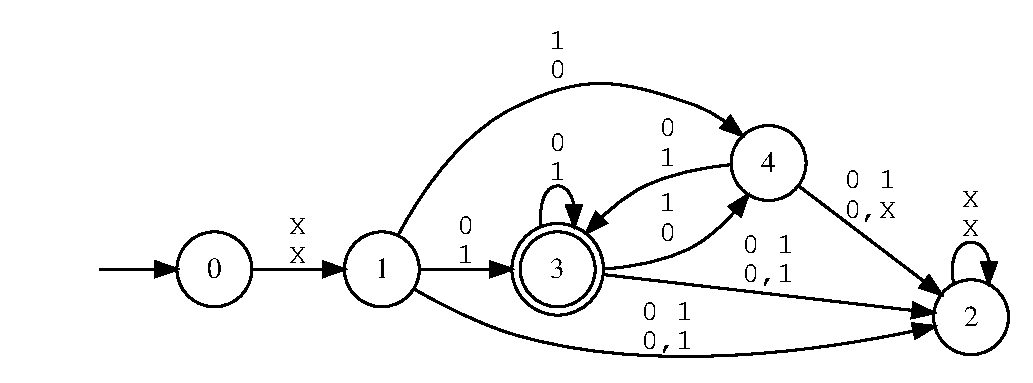
\includegraphics[width=\linewidth]{images/pre-automaton.eps}
  \caption{The \DFA output from \MONA}
  \label{fig:mona-output}
\end{subfigure}%
\begin{subfigure}{.5\textwidth}
  \centering
  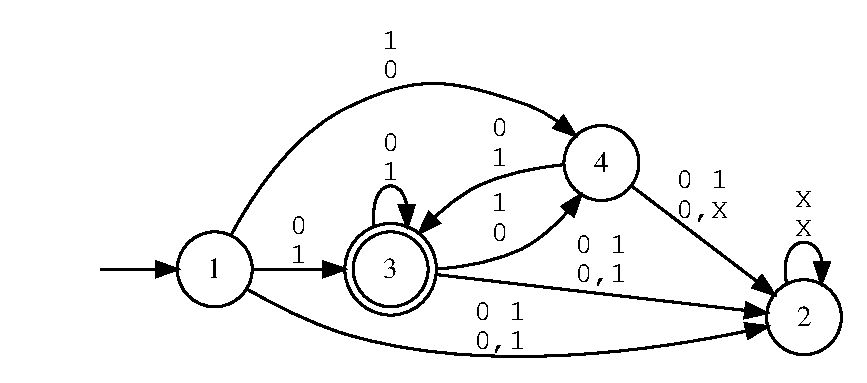
\includegraphics[width=\linewidth]{images/post-automaton.eps}
  \caption{The \DFA post-processed}
  \label{fig:automa-post-processed}
\end{subfigure}
\caption{Before and after \DFA post-processing}
\label{fig:pre-post-automaton}
\end{figure}
\section{Comparison with \FLLOAT}
\section{Discussion}
In this chapter, we have presented the \LTLfToDFA Python package. We have also described the structure of the package, discussed in detail its implementation highlighting all the main features and, finally, seen how it performs with respect to time and memory relatively to the \FLLOAT Python package.


















